\input{configuration}

\title{Lecture 22 --- Kernel Modules and eBPF}

\author{Jeff Zarnett \\ \small \texttt{jzarnett@uwaterloo.ca}}
\institute{Department of Electrical and Computer Engineering \\
  University of Waterloo}
\date{\today}


\begin{document}

\begin{frame}
  \titlepage
\end{frame}



\begin{frame}
\frametitle{New Functionality}

A modern general-purpose operating system needs to be able to adapt/change.

Example: supporting new devices. Now we can add new kernel functionality.

\begin{center}
	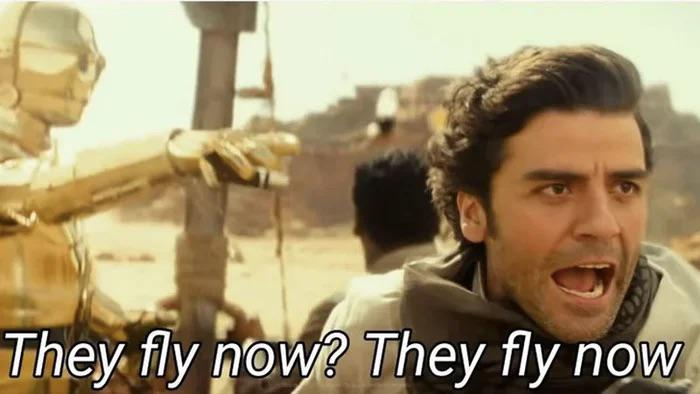
\includegraphics[width=0.4\textwidth]{images/theyflynow.jpg}
\end{center}

\end{frame}


\begin{frame}
\frametitle{Loading and Unloading}

Modern kernels permit the ability to load and unload pieces of functionality through the use of \alert{modules}, which are exactly what they sound like.

Self-contained chunks of code that can become part of the kernel. 

The additional code can be loaded at boot up, or dynamically on request, and unloaded (disabled) if no longer needed.

\end{frame}


\begin{frame}
\frametitle{Using it for What?}

One popular usage of kernel modules is anti-cheating software in online games. 

\begin{center}
	
\includegraphics[width=0.55\textwidth]{images/anticheat.jpg}
\end{center}

\end{frame}


\begin{frame}
\frametitle{Anti-Cheat}

Why would a game need to load a kernel module to reduce cheating?! 

\end{frame}

\begin{frame}
\frametitle{Fight Fire with Fire}

Regardless of how you feel about the ethics of cheating in online multiplayer games, some players are \textit{extremely} dedicated to winning at all costs.

Competitive games are not very much fun when other players cheat.\\
\quad The game needs to use every mechanism available to the would-be cheaters.

Fight fire with fire, as it were.

\end{frame}


\begin{frame}
\frametitle{Example: Wallhack}

\begin{center}
	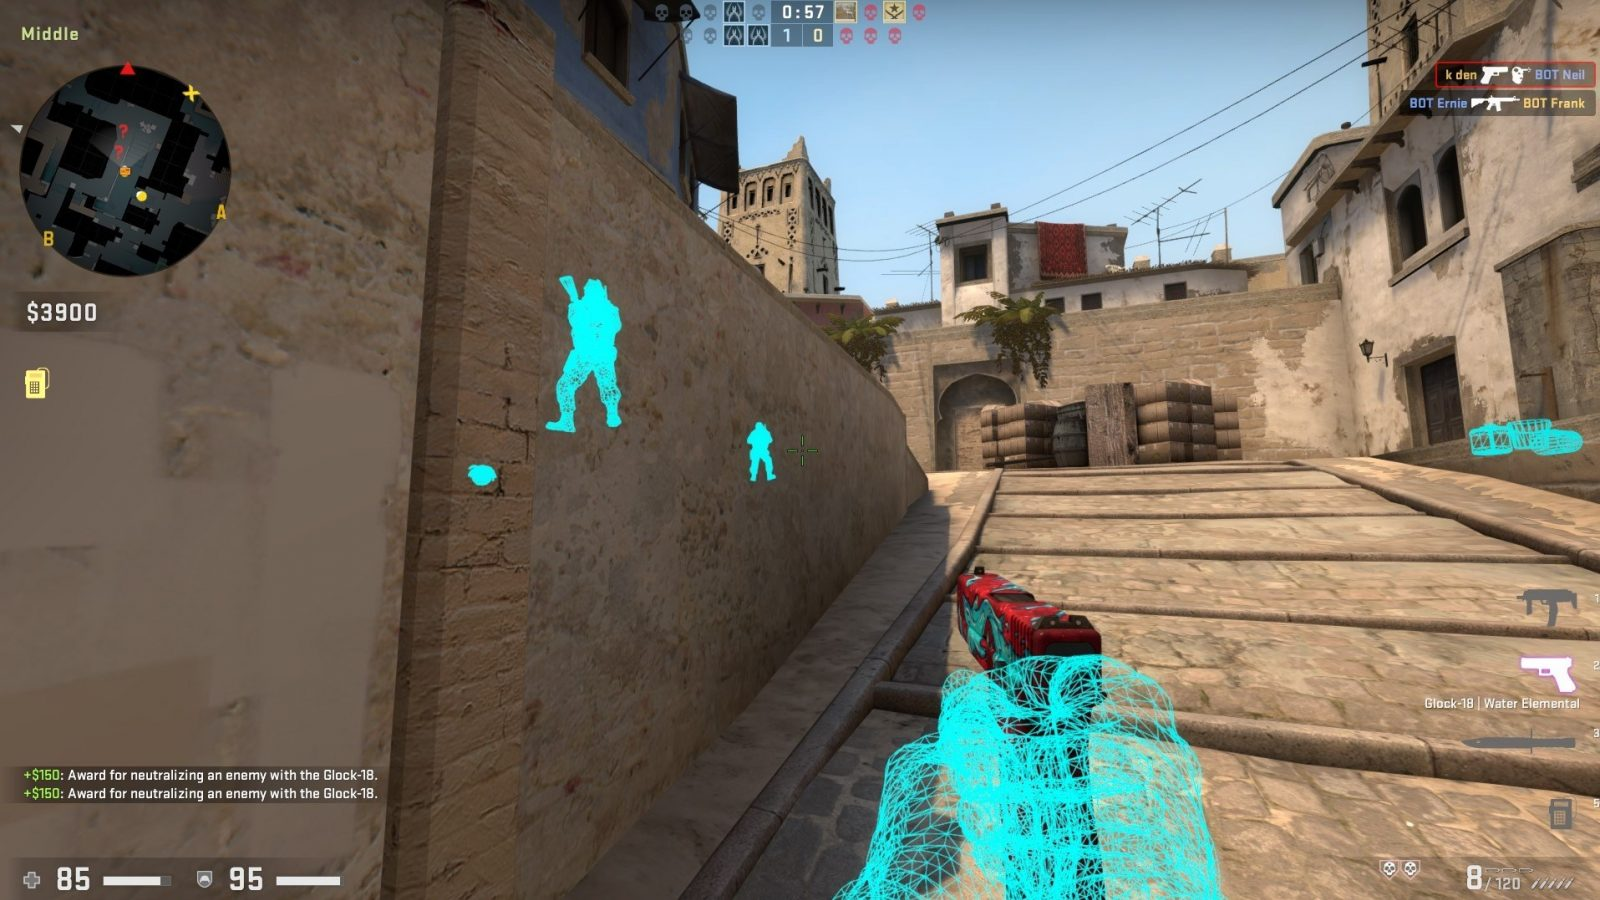
\includegraphics[width=0.85\textwidth]{images/wallhack.jpg}
\end{center}


\end{frame}


\begin{frame}
\frametitle{Specific Kernel}

Kernel modules are specific to a given kernel.


This is a part of the reason why it can be difficult to play games on Linux.

Of course, there are numerous other reasons for kernel modules aside from just anti-cheating. Let's move on to the mechanics: how do we create and load them?

\end{frame}


\begin{frame}
\frametitle{Creating a Module}


Writing kernel modules comes with a number of differences! 

For example, the kernel defines a \texttt{linux/printk.h} header that lets us use the \texttt{pr\_info()} macro to print -- something we would normally do with \texttt{printf}.

The kernel must be able to run without the standard C library.

Similarly, if you need to allocate memory, there are kernel-specific functions like \texttt{kmalloc} to accomplish what you want -- a regular \texttt{malloc} will not work. 

\end{frame}


\begin{frame}
\frametitle{Getting Started}

A kernel module has an initialization function that is run on loading the module and a cleanup function that is run to clean up when an unload is taking place.

These used to be called \texttt{init\_module()} and \texttt{cleanup\_module()}.

More modern versions of the kernel permit you to call them anything as long as they are registered with the macros.
\end{frame}


\begin{frame}[fragile]
\frametitle{Hello World Module}

\begin{lstlisting}[language=C]
#include <linux/init.h> /* Needed for the macros */
#include <linux/module.h> /* Needed by all modules */
#include <linux/printk.h> /* Needed for pr_info() */

static int __init hello_2_init(void)
{
    pr_info("Hello, world 2\n");
    return 0;
}

static void __exit hello_2_exit(void)
{
    pr_info("Goodbye, world 2\n");
}

module_init(hello_2_init);
module_exit(hello_2_exit);

MODULE_LICENSE("GPL");
\end{lstlisting}

A more complex kernel module must account for concurrency and use concurrency-control constructs.

\end{frame}


\begin{frame}
\frametitle{System Call Changes}

It sounds like we now have a clear pathway to add a system call. 

In discussing how they worked much earlier on, we said that an integer identifier was put in a predefined location and the trap instruction invoked, which activated the OS. 

The OS then looks at the identifier and uses that to make a determination of what system call handler to run. 

\end{frame}

\begin{frame}
\frametitle{System Call Changes}

So if you want to add a new system call? 

We just need to bring the new code into the kernel and then update the mapping table so that the new number has a corresponding handler function to run. 

To replace one? Bring in the new code and then update the mapping table so the existing number points to the new function instead of the old one.

\end{frame}


\begin{frame}
\frametitle{There's Only One Problem}

\begin{center}
	
\includegraphics[width=0.5\textwidth]{images/handonshoulder.jpg}
\end{center}

The kernel maintainers broke this as collateral damage of a security mitigation.

\end{frame}


\begin{frame}
\frametitle{Upkeep}

Earlier, it was mentioned that modules are specific to a given kernel.  

This is because the kernel itself has no stable internal API. 

Yes, Linus Torvalds gets extremely mad if a change breaks a user program! 

Internally the kernel data structures, functions and their signatures, and everything else can change arbitrarily at any time. 

\end{frame}


\begin{frame}
\frametitle{Why Internals are Unstable}


\begin{enumerate}
	\item[1.] \textbf{Binary Interface.} The compiled binary of the kernel does not remain consistent from build to build for a few reasons:
		\begin{itemize}
			\item Changes to the C compiler can result in different binary output.
			\item Build options can change what \texttt{struct}s look like or what function implementation blocks appear, and memory alignment.
			\item The kernel runs on different architectures (e.g., x86\_64, arm).
		\end{itemize}
\end{enumerate}

\end{frame}


\begin{frame}
\frametitle{Why Internals are Unstable}

\begin{enumerate}
	\item[2.] \textbf{Source Interfaces.} The API of the kernel can change too. This is a design decision that gives a high degree of freedom to kernel developers to do things:
		\begin{itemize}
			\item Fix a bug or improve a design decision without needing to support backwards-compatibility.
			\item Retire an old implementation in favour of a new and ostensibly better implementation, also without worrying about backwards-compatibility.
			\item Address security issues without having the same constraints about breaking things we discussed in the introduction to the course.
		\end{itemize}
\end{enumerate}

\end{frame}


\begin{frame}
\frametitle{Get It In}

The fact that these internal interfaces and data structures can change at any time pushes contributors to try to get their code included into the kernel source itself.


High standards for getting things accepted into the Kernel!
\end{frame}


\begin{frame}
\frametitle{You Sure About This?}

Should we implement something as a kernel module?\\
\quad It is truly dangerous to do so.

\begin{center}
	
\includegraphics[width=0.4\textwidth]{images/thedanger.jpg}
\end{center}

The kernel has effectively unlimited ability to do anything in the system.

\end{frame}


\begin{frame}
\frametitle{Signing Modules}
Linux offers the ability to cryptographically sign modules to verify that they come from the source that they claim to come from. 

Whether users actually check the signatures or just override and say install anyway is a different matter.

 It is possible to configure the kernel to reject unsigned modules. 

\end{frame}


\begin{frame}
\frametitle{Crowdstrike Outage}

\begin{center}
	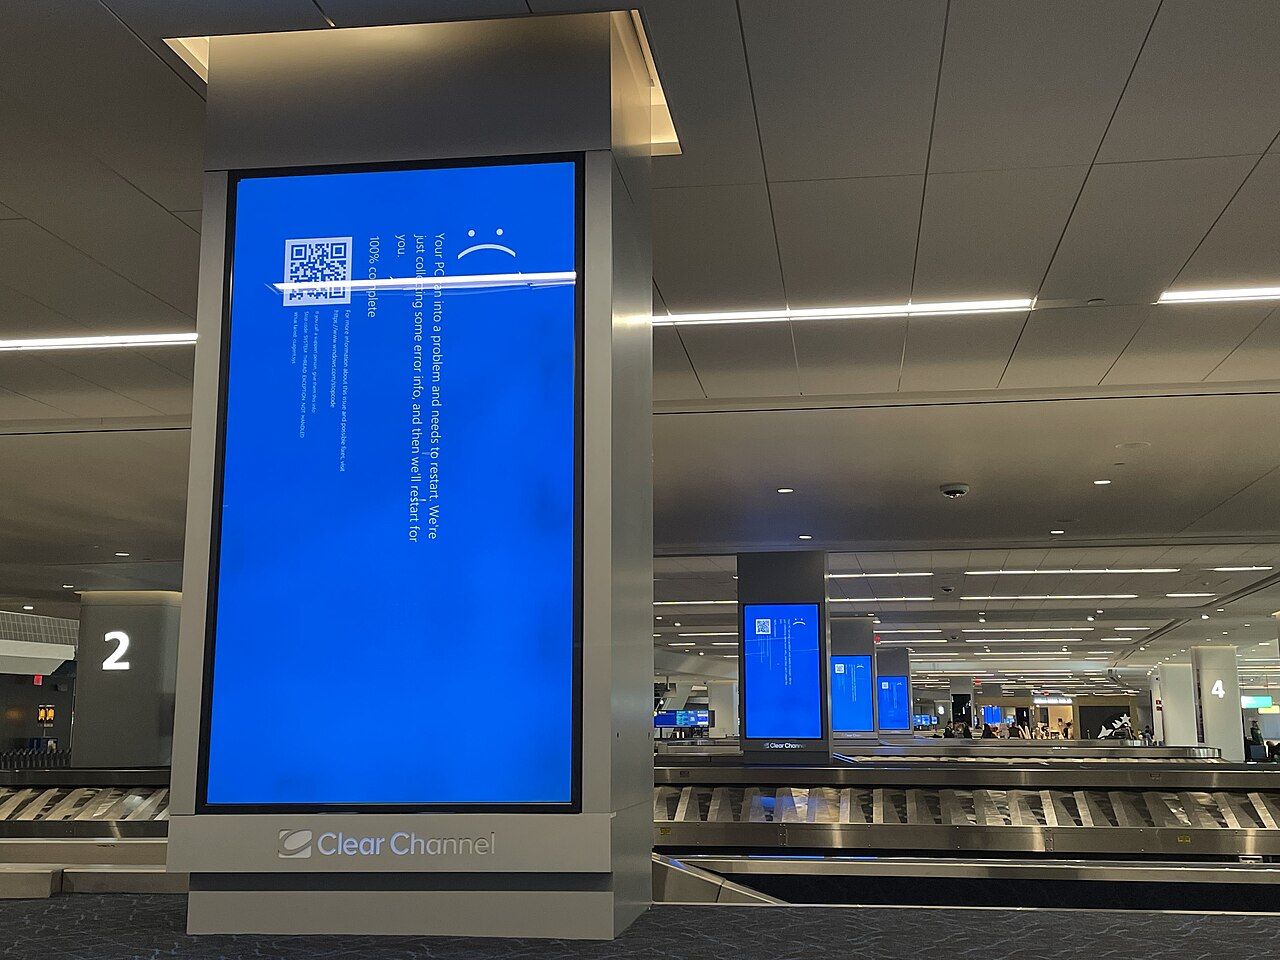
\includegraphics[width=0.8\textwidth]{images/crowdstrike-bsod.jpg}
\end{center}

On July 19, 2024, an update to a kernel module configuration from CrowdStrike caused a huge number of Windows machines to experience the BSOD.

\end{frame}


\begin{frame}
\frametitle{Crowdstrike Outage}

Was the CrowdStrike driver signed? Yes!

 Microsoft also has the ability to sign kernel extensions and the one that caused the incident was signed. 
 
 The configuration change itself is unverified but it does get imported by something that is. 
 
 There could not be a clearer indication that the signing of a module simply proves where it comes from and is not a guarantee of quality or correctness.

\end{frame}


\begin{frame}
\frametitle{eBPF}

Idea: extend the kernel without changing the source or loading modules.

The eBPF approach is to execute a program at designated hooks inside the kernel.

What are hooks? 


\end{frame}


\begin{frame}
\frametitle{eBPF Hooks}

When the kernel is executing, if it passes a certain point, such as the start of a system call or entry/exit of a function, then that can be the trigger to run the eBPF program. 

That code runs and then the kernel function executes as normal afterwards.

\end{frame}

\begin{frame}
\frametitle{eBPF Hook}

\begin{center}
	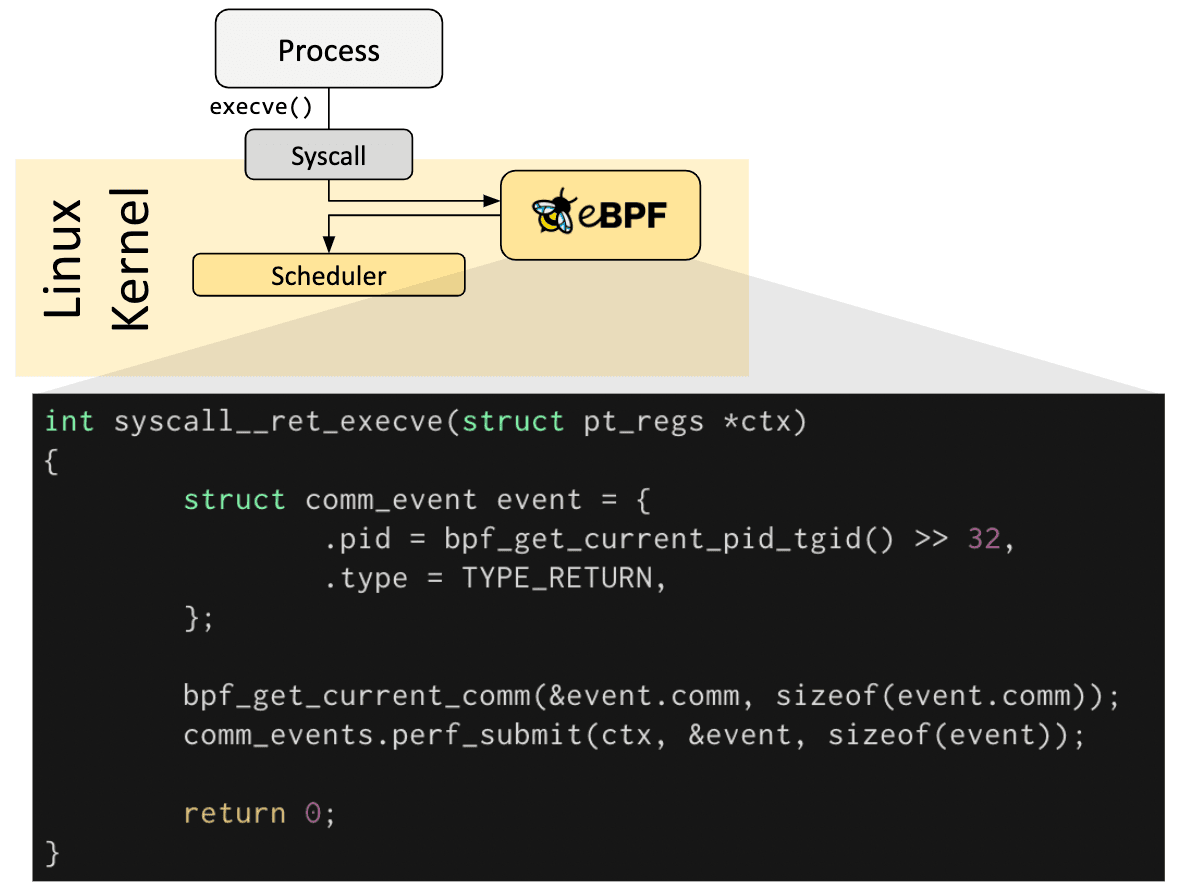
\includegraphics[width=0.8\textwidth]{images/syscall-hook.png}
\end{center}

\end{frame}


\begin{frame}
\frametitle{Verification}

Verification is interesting! 

The eBPF verifier does a static (load time) analysis of the byte code to determine if it is ``safe'' to run.

If it passes then it goes to a just-in-time compiler and the output is the machine code that actually runs.

\end{frame}


\begin{frame}
\frametitle{Verification}

The documentation summarizes the verification as saying that it checks:

\begin{enumerate}
	\item If the process loading the program has the capabilities needed to execute it.
	\item That the program does not crash or cause any other harm.
	\item That the program runs to completion (no infinite loop).
\end{enumerate}

\end{frame}


\begin{frame}
\frametitle{How Sure is Sure?}

You would be right to question whether the verification actually demonstrates that the code is safe. 

Any verification process is also software, and software has bugs. 

So the verifier can make mistakes too, and may say yes to a program that has a problem or no to one that should be approved. 

Still, the existence of verification suggests at least a higher chance of staying out of trouble.

\end{frame}


\begin{frame}
\frametitle{eBPF like JavaScript}

The documentation of eBPF compares the utility of this tool as being like JavaScript in the browser.

JS permits a website to be as dynamic and app-like as you want, because JavaScript can run arbitrary code.

It's in a sandbox of sorts, and the website can update itself whenever it is ready rather than needing a browser update. 

\end{frame}


\begin{frame}
\frametitle{Verification and Compilation}

After verification is completed, there's the compilation process. 

The compilation process is just-in-time (on the fly) and it involves an optimization pass that removes dead or unreachable code before turning it into the binary.

Why would there be dead code? The answer has to do with portability.

\end{frame}


\begin{frame}
\frametitle{Portability}

The kernel module discussion covers clearly that upkeep of a kernel module is challenging because the kernel internals can change at any time. 

Programs loaded via eBPF also have this problem, if they look at kernel data structures or use kernel functions. 

If the name of the structure has changed, for example, the eBPF program will be looking at the wrong thing. 

\end{frame}


\begin{frame}[fragile]
\frametitle{Simple Case: New Variable Name}
\begin{lstlisting}[language=C]
extern u32 LINUX_KERNEL_VERSION __kconfig;
extern u32 CONFIG_HZ __kconfig;

u64 utime_ns;

if (LINUX_KERNEL_VERSION >= KERNEL_VERSION(4, 11, 0))
    utime_ns = BPF_CORE_READ(task, utime);
else
    /* convert jiffies to nanoseconds */
    utime_ns = BPF_CORE_READ(task, utime) * (1000000000UL / CONFIG_HZ);
\end{lstlisting}

\end{frame}


\begin{frame}
\frametitle{New Function}

If the function \texttt{work2()} has been introduced in some new kernel version, then we can start using that and use \texttt{work1()} in the old version, right? 

Yes, except what if \texttt{work1()} has been removed from the kernel?

The if-else logic still contains a reference to \texttt{work1()} and the compiler will not find it and that should fail the compilation. 

This is why the eBPF approach does the optimization pass to remove dead code.


\end{frame}


\begin{frame}[fragile]
\frametitle{Complex Scenario: Structure Changes}

\begin{lstlisting}[language=C]
/* up-to-date thread_struct definition matching newer kernels */
struct thread_struct {
    ...
    u64 fsbase;
    ...
};

/* legacy thread_struct definition for <= 4.6 kernels */
struct thread_struct___v46 { /* ___v46 is a "flavor" part */
    ...
    u64 fs;
    ...
};

extern int LINUX_KERNEL_VERSION __kconfig;
...
struct thread_struct *thr = ...;
u64 fsbase;
if (LINUX_KERNEL_VERSION < KERNEL_VERSION(4, 7, 0))
    fsbase = BPF_CORE_READ((struct thread_struct___v46 *)thr, fs);
else
    fsbase = BPF_CORE_READ(thr, fsbase);
\end{lstlisting}

Three underscores mean this is a \alert{flavour}.

The alternative to this flavour approach would be lots of \texttt{\#ifdef} kind of blocks.

\end{frame}



\begin{frame}
\frametitle{Game On}

This topic opened by looking at anti-cheat kernel modules, so the obvious example of using eBPF is also gaming-related!

It is the \texttt{scx\_lavd} (Latency-criticality Aware Virtual Deadline) scheduling algorithm.

Used by the Steam Deck!

\end{frame}


\begin{frame}
\frametitle{Using eBPF For Scheduling}

This is a possibility because the kernel introduced a new scheduler class (\texttt{sched\_ext}) that permits a BPF program to take on the role of scheduling for threads in this class. 

Kernel docs: ``detection of any internal error including stalled runnable tasks aborts the BPF scheduler and reverts all tasks back to the fair-class scheduler''. 

This is another point for safety of using the eBPF approach: if anything goes wrong, the system reverts back to the default scheduler.

\end{frame}


\begin{frame}
\frametitle{LAVD Goals}

The LAVD scheduler balances two goals: gaming experience and energy efficiency. 

Gaming experience is shaped by two things, the average Frames Per Second (FPS) but also ``stuttering''. 

It's a deadline-based scheduling algorithm.

\end{frame}


\begin{frame}
\frametitle{LAVD}

To actually implement it, a small amount of Rust code is needed (outside kernel).

Is this a sensible approach? I would argue yes.

This scheduler is somewhat niche and not right for all workloads.

\end{frame}



\end{document}
